% Options for packages loaded elsewhere
\PassOptionsToPackage{unicode}{hyperref}
\PassOptionsToPackage{hyphens}{url}
\documentclass[
  twocolumn]{article}
\usepackage{xcolor}
\usepackage[margin=1in]{geometry}
\usepackage{amsmath,amssymb}
\setcounter{secnumdepth}{-\maxdimen} % remove section numbering
\usepackage{iftex}
\ifPDFTeX
  \usepackage[T1]{fontenc}
  \usepackage[utf8]{inputenc}
  \usepackage{textcomp} % provide euro and other symbols
\else % if luatex or xetex
  \usepackage{unicode-math} % this also loads fontspec
  \defaultfontfeatures{Scale=MatchLowercase}
  \defaultfontfeatures[\rmfamily]{Ligatures=TeX,Scale=1}
\fi
\usepackage{lmodern}
\ifPDFTeX\else
  % xetex/luatex font selection
\fi
% Use upquote if available, for straight quotes in verbatim environments
\IfFileExists{upquote.sty}{\usepackage{upquote}}{}
\IfFileExists{microtype.sty}{% use microtype if available
  \usepackage[]{microtype}
  \UseMicrotypeSet[protrusion]{basicmath} % disable protrusion for tt fonts
}{}
\makeatletter
\@ifundefined{KOMAClassName}{% if non-KOMA class
  \IfFileExists{parskip.sty}{%
    \usepackage{parskip}
  }{% else
    \setlength{\parindent}{0pt}
    \setlength{\parskip}{6pt plus 2pt minus 1pt}}
}{% if KOMA class
  \KOMAoptions{parskip=half}}
\makeatother
\usepackage{graphicx}
\makeatletter
\newsavebox\pandoc@box
\newcommand*\pandocbounded[1]{% scales image to fit in text height/width
  \sbox\pandoc@box{#1}%
  \Gscale@div\@tempa{\textheight}{\dimexpr\ht\pandoc@box+\dp\pandoc@box\relax}%
  \Gscale@div\@tempb{\linewidth}{\wd\pandoc@box}%
  \ifdim\@tempb\p@<\@tempa\p@\let\@tempa\@tempb\fi% select the smaller of both
  \ifdim\@tempa\p@<\p@\scalebox{\@tempa}{\usebox\pandoc@box}%
  \else\usebox{\pandoc@box}%
  \fi%
}
% Set default figure placement to htbp
\def\fps@figure{htbp}
\makeatother
\setlength{\emergencystretch}{3em} % prevent overfull lines
\providecommand{\tightlist}{%
  \setlength{\itemsep}{0pt}\setlength{\parskip}{0pt}}
\usepackage{longtable}
\usepackage{etoolbox}
\usepackage[T1]{fontenc} \usepackage[utf8]{inputenc} \usepackage[portuguese]{babel} \usepackage{booktabs} \usepackage{float} \usepackage{graphicx}
\usepackage{booktabs}
\usepackage{longtable}
\usepackage{array}
\usepackage{multirow}
\usepackage{wrapfig}
\usepackage{float}
\usepackage{colortbl}
\usepackage{pdflscape}
\usepackage{tabu}
\usepackage{threeparttable}
\usepackage{threeparttablex}
\usepackage[normalem]{ulem}
\usepackage{makecell}
\usepackage{xcolor}
\usepackage{bookmark}
\IfFileExists{xurl.sty}{\usepackage{xurl}}{} % add URL line breaks if available
\urlstyle{same}
\hypersetup{
  pdftitle={Relatorio},
  pdfauthor={Fabio Firanzi, Heitor Dias, Julia Fideles, Matheus Soares, Tiago Braga},
  hidelinks,
  pdfcreator={LaTeX via pandoc}}

\title{Relatorio}
\author{Fabio Firanzi, Heitor Dias, Julia Fideles, Matheus Soares, Tiago
Braga}
\date{2025-11-11}

\begin{document}
\maketitle

\begin{tabular}{llr}
\toprule
Presença na prova & Percentual & Frequência\\
\midrule
Ausente & 26.74\% & 115880\\
Presente & 73.12\% & 316843\\
Eliminado & 0.13\% & 571\\
\bottomrule
\end{tabular}

\includegraphics[width=\linewidth]{relatorio_files/figure-latex/grafico-presenca-1}

\section{Tabela e gráfico de
presença}\label{tabela-e-gruxe1fico-de-presenuxe7a}

A tabela ``Frequência de presença na prova de LC'' e o Gráfico
``Presença na prova de LC'' exibem a porcentagem de alunos presentes,
ausentes e eliminados na prova de linguágens e códigos. Com base nessa
tabela, pode-se identificar que a grande maioria, 73,1\%, dos alunos
estava presente na avaliação, 26,7\% ausente e uma minoria de 0,1\% foi
eliminada antes, durante ou após a prova. Embora a maioria tenha
completado a avaliação, o alto índice de ausência sugere a necessidade
de estudos futuros para investigar os fatores que contribuem para essa
abstenção.

\includegraphics[width=\linewidth]{relatorio_files/figure-latex/hist-linguagens-1}

\section{Histograma da nota de LC}\label{histograma-da-nota-de-lc}

Para a criação desse histograma foi utilizado a nota dos alunos
presentes e não eliminados na avaliação de Linguagens e códigos, com
esse dado sendo analizado em sua frequência, média, desvio padrão e
distribuição.

O ``Histograma da Nota de LC'' ilustra a distribuição de frequência das
notas de Linguagens e Códigos para todos os alunos presentes. Ele foi
construído sobrepondo uma curva normal teórica (linha vermelha),
calculada a partir da média e do desvio padrão da amostra, sobre o
histograma das notas reais (barras azuis).

A maior concentração de notas é de 500-600 pontos, contendo
aproximadamente 55\% dos alunos, o desvio padrão das notas é de 69,87.

\begin{table}
\centering
\caption{\label{tab:unnamed-chunk-2}Tabela Comparativa: LC vs MT (para 298.976 alunos presentes em ambas e com nota > 0)}
\centering
\begin{tabular}[t]{lrrrrr}
\toprule
Prova & Média & Mediana & Desv. Padrão & Min & Máx\\
\midrule
LC & 526.70 & 533.3 & 68.03 & 298.8 & 795.8\\
MT & 527.24 & 499.1 & 113.91 & 342.8 & 961.9\\
\bottomrule
\end{tabular}
\end{table}

\section{Tabela e gráfico LC vs MT}\label{tabela-e-gruxe1fico-lc-vs-mt}

A tabela ``Tabela comparativa: LC vs MT'' ilustra as, médias, medianas,
desvios-padrão, notas mínimas e notas máximas das provas de linguagens e
matemática, considerando apenas os alunos que estiveram presentes em
ambas delas.

O gráfico ``comparação das distribuições de notas:LC vs MT'' exibe os
gráficos de distribuição de notas de linguagens e matemática
sobrepostos, oferecendo uma comparação visual direta e clara da
distribuição de notas das duas matérias.

Embora as médias de linguagens e matemática tenham sido muito próximas,
526,7 e 527,2 respectivamente, a distribuição de notas da prova de
matemática é totalmente diferente da de linguagens (que se aproxima de
uma normal perfeita) tendo suas notas muito mais distribuidas no
gráfico, evidenciando um desvio padrão muito maior.

\pandocbounded{\includegraphics[keepaspectratio]{relatorio_files/figure-latex/Gráfico de Densidade LC vs MT-1.pdf}}

O Gráfico de Densidade oferece uma comparação visual direta entre as
distribuições das notas de Linguagens (vermelho) e Matemática (azul).
Este gráfico foi gerado utilizando apenas os alunos que compareceram e
obtiveram nota maior que zero em ambas as provas. Percebe-se que a curva
de Matemática é mais achatada e espalhada (refletindo o maior desvio
padrão), indicando que há uma variabilidade muito maior nas notas. Em
contraste, as notas de Linguagens são mais ``pontudas'' e concentradas
em torno de sua média.

\pandocbounded{\includegraphics[keepaspectratio]{relatorio_files/figure-latex/boxplot-nota-regiao-1.pdf}}

O Boxplot complementa a tabela estatística anterior, visualizando a
distribuição das notas de Linguagens e Códigos por região. Ele foi
criado agrupando os alunos por região e ordenando o eixo Y pela mediana
das notas, da maior para a menor. Este gráfico permite uma visualização
clara não apenas da mediana (a linha central na caixa), mas também da
dispersão do ``meio'' dos alunos (o tamanho da caixa, ou Intervalo
Interquartil) e dos outliers (pontos). Observa-se que as regiões Sudeste
e Sul apresentam as medianas mais elevadas, enquanto as regiões Nordeste
e Norte mostram um desempenho mediano inferior e uma dispersão de notas
(tamanho da caixa) ligeiramente maior, indicando maior variação no
desempenho dos alunos dessas regiões.

\begin{table}
\centering
\begin{tabular}{lrrrrrrr}
\toprule
Região & Média & Mediana & Var & D. Padrão & Min & Máx & Nº de Alunos\\
\midrule
S & 542.13 & 548.0 & 3935.23 & 62.73 & 298.8 & 795.8 & 141162\\
CO & 527.52 & 533.5 & 4542.66 & 67.40 & 298.8 & 777.4 & 24755\\
NE & 510.60 & 516.3 & 4889.35 & 69.92 & 298.8 & 795.8 & 116314\\
N & 499.47 & 505.4 & 4805.12 & 69.32 & 298.8 & 732.3 & 34406\\
\bottomrule
\end{tabular}
\end{table}

\section{Tabela e boxplot de notas LC por
região}\label{tabela-e-boxplot-de-notas-lc-por-regiuxe3o}

A tabela ``Estatísticas das notas de LC por Região'' exibe as médias,
medianas, variências, desvios-padrão, notas mínimas, notas máximas e
número aproximado de alunos de cada região do Brasil.

O ``Boxplot das notas de linguagens por Região'', ilustra a performance
dos alunos de cada uma das regiões do Brasil exibindo a distribuição das
notas. As ``caixas'' representam os 50\% centrais dos alunos, com os
pontos sendo os ``outliers'', ou seja, os fora da média, tanto para
baixo quanto para cima e a linha dentro da caixa representa a mediana.
Com base no boxplot, a região Sudoeste obteve o melhor resultado, com
sua média de 542,74 sendo a mais alta seguida de perto pela região Sul e
sua média de 540.36, o boxplot também deixa evidente a desigualdade do
país, com as regiões Norte e nordeste ficando significativamente atras
das demais.

\section{Analise da variavel de presença na prova de
humanas}\label{analise-da-variavel-de-presenuxe7a-na-prova-de-humanas}

Foi feita uma analise da area de conhecimento de Ciências Humanas do
Enem, utilizando a varivel: TP\_PRESENCA\_CH. Tal variavel, é
classificada como qualitativa possuindo 3 possíveis valores:

\begin{itemize}
\tightlist
\item
  0: Ausente
\item
  1: Presente
\item
  2: Eliminado da Prova
\end{itemize}

\subsection{Gráfico de Frequências das presenças no dia da
prova}\label{gruxe1fico-de-frequuxeancias-das-presenuxe7as-no-dia-da-prova}

Busca indentificar se o aluno estava presente, ausente ou se foi
eliminado da prova de ciências humanas, e, com isso, expressar a
porcentagem e os valores absolutos da variável TP\_PRESENCA\_CH.

\pandocbounded{\includegraphics[keepaspectratio]{relatorio_files/figure-latex/analise_variavel_presenca-1.pdf}}
O gráfico ``Percentual de Presença na Prova de CH'', trata dos dados da
variável `TP\_PRESENCA\_CH'. Uma vez que a variável é do tipo
qualitativa, a abordagem mais convencional é um gráfico de barras dos
percentuais.

Com base na analise do gráfico ``Percentual de Presença na Prova CH''
foi possível determinar que no Exame Nacional do Ensino Médio (ENEM),
edição de 2024, o número de alunos presentes foi de aproximadamente 2,73
vezes maior que o número de alunos ausentes. Além disso, percebe-se que
a quantidade de alunos elimanados na prova de Ciências Humanas foi
extremamente pequena - 0,1\% - comparado com os percentuais da coluna
``Presença'' e da coluna ``Ausente''.

\section{Analise da variavel Notas da prova de Ciências
Humanas}\label{analise-da-variavel-notas-da-prova-de-ciuxeancias-humanas}

\begin{table}[!h]
\centering
\caption{\label{tab:analise-medidas-estatistica}Tabela Resumo: Estatísticas das Notas de CH por Região}
\centering
\resizebox{\ifdim\width>\linewidth\linewidth\else\width\fi}{!}{
\begin{tabular}[t]{lrrrrrr}
\toprule
Regiao & Media & Mediana & Variancia & Desvio Padrao & Minimo & Maximo\\
\midrule
\cellcolor{gray!10}{Sudeste} & \cellcolor{gray!10}{533.58} & \cellcolor{gray!10}{540.4} & \cellcolor{gray!10}{7482.78} & \cellcolor{gray!10}{86.50} & \cellcolor{gray!10}{283.8} & \cellcolor{gray!10}{819.7}\\
Sul & 527.92 & 534.0 & 7095.26 & 84.23 & 283.8 & 819.7\\
\cellcolor{gray!10}{Centro-Oeste} & \cellcolor{gray!10}{514.69} & \cellcolor{gray!10}{518.7} & \cellcolor{gray!10}{8192.05} & \cellcolor{gray!10}{90.51} & \cellcolor{gray!10}{283.8} & \cellcolor{gray!10}{817.4}\\
Nordeste & 495.07 & 494.9 & 8216.95 & 90.65 & 283.8 & 819.7\\
\cellcolor{gray!10}{Norte} & \cellcolor{gray!10}{484.05} & \cellcolor{gray!10}{481.2} & \cellcolor{gray!10}{7511.50} & \cellcolor{gray!10}{86.67} & \cellcolor{gray!10}{283.8} & \cellcolor{gray!10}{808.2}\\
\bottomrule
\end{tabular}}
\end{table}

A ``Tabela Resumo: Estatísticas das Notas de CH por Região'' apresenta a
distribuição das medidas: media,mediana, variância, desvio padrão, valor
mínimo, valor máximo e a frequência relativa percentual. Essa divisão
foi feita por região do Brasil. Com base nisso, podemos identificar
claramente o desempenho superior da região Sudeste.

Liderança Clara: O Sudeste lidera em ambos os indicadores de
performance, possuindo a maior Média (593,12) e, mais importante, a
maior Mediana (601,8).

O ``Grupo de Ponta'': Embora o Sudeste seja o primeiro, ele faz parte de
um ``grupo de alta performance'' juntamente com as regiões Sul (Mediana
597,5) e Centro-Oeste (Mediana 591,3). Estas três regiões estão
claramente destacadas das regiões Nordeste (Mediana 562,9) e Norte
(Mediana 555,0).

A Armadilha da Média: Em todas as regiões, a Média é ``puxada'' para
baixo por notas mais fracas (assimetria à esquerda). Por isso, a Mediana
é a métrica mais justa para a comparação, e nela o Sudeste também vence.

\subsection{Gráfico Boxplot da variável
notas}\label{gruxe1fico-boxplot-da-variuxe1vel-notas}

\pandocbounded{\includegraphics[keepaspectratio]{relatorio_files/figure-latex/grafico_boxplot_regiao_COMPLETO-1.pdf}}

O gráfico ``Boxplot das Notas de CH por Região'', compara o desempenho
central (a mediana) das notas de Ciências Humanas (CH) entre as cinco
grandes regiões do Brasil. Além disso, o gráfico representa os valores
``extremos'', os outliers, da variavel `NU\_NOTA\_CH', contribuindo para
uma analise de desempenho na prova do Enem.

As caixas das regiões Sul e Sudeste são visivelmente mais longas
(largas) do que as das outras regiões. Isto significa que a diferença de
nota entre o aluno do percentil 25 e o do percentil 75 é maior. Ou seja,
embora tenham o melhor desempenho, são regiões internamente mais
``desiguais'' ou ``inconstantes''.

O Boxplot confirma que a região Sudeste tem o melhor desempenho geral em
Ciências Humanas, não apenas na mediana, mas no ``corpo'' principal dos
seus alunos (o miolo de 50\%). No entanto, esta alta performance vem
acompanhada de uma maior desigualdade interna (maior dispersão)
representada pelo comprimento maior e um alto número de Outliers, tanto
Outliers superiores (notas \textgreater{} 750) quanto os Outliers
inferiores (notas \textless{} 300), um padrão também visto na região
Sul.

\subsection{Histograma de Densidade com Média e Desvio
Padrão}\label{histograma-de-densidade-com-muxe9dia-e-desvio-padruxe3o}

Para os dados quantitativos contínuos da variável NU\_NOTA\_CH, que
representa as notas dos alunos na prova de ciências humanas, criamos
classes (faixas de valores) para a desenvolver um histograma com uma
Normal sobreposta.

\pandocbounded{\includegraphics[keepaspectratio]{relatorio_files/figure-latex/chunk-grafico-densidade-percentual-1.pdf}}
O ``Histograma de Densidade com Média e Desvio Padrão'' apresenta a
densidade das notas de Ciências Humanas (CH), indicando a distribuição
dos valores observados. As barras em azul representam a frequência
relativa das notas, enquanto a linha vermelha mostra a curva normal
teórica ajustada a partir dos dados. Além disso, a linha pontilhada
vertical identifica a média das notas (510,92 pontos). Nesse cenário,
essa variavel possui O desvio-padrão igual a 92,95 pontos, informado no
canto superior direito do gráfico. Todos esses fatores auxiliam para a
execução de uma analise a cerca da distribuição das notas da prova de
Ciências Humanas.

A faixa de nota com maior frequência (a Classe Modal) é {[}500, 550),
contendo 21.05\% dos alunos.

As notas de Ciências Humanas apresentam uma distribuição aproximadamente
normal, bem representada pela curva teórica sobreposta ao histograma. A
média foi de 510,92 pontos, indicando o desempenho central dos
estudantes, enquanto o desvio-padrão de 92,95 pontos mostra dispersão
moderada ao redor da média. A forma da distribuição confirma que os
dados seguem um padrão típico e estável, adequado para análises baseadas
em normalidade.

\section{1.3 Correlação e Regressão Linear
Simples}\label{correlauxe7uxe3o-e-regressuxe3o-linear-simples}

Para essa analise, buscou-se indentificar o poder de correlação de duas
variaveis, notas de Ciências Humanas e notas de Linguagens e Códigos.

Nesta análise, vamos investigar a relação entre duas variáveis
quantitativas: NU\_NOTA\_LC (Linguagens e Códigos) e NU\_NOTA\_CH
(Ciências Humanas).

\begin{itemize}
\item
  Variável Independente (X): NU\_NOTA\_LC
\item
  Variável Dependente (Y): NU\_NOTA\_CH
\end{itemize}

O objetivo é responder: ``A nota de Linguagens pode prever a nota de
Humanas?''

Para isso, foi feita um processo de filtragem, matendo somente os alunos
com notas válidas (sem N) e os alunos com notas maiores que zero em
ambas as variaveis. Com isso, o número total de observações válidas para
a regressão: foi de 316201.

\subsection{Coeficiente de Correlação de
Pearson}\label{coeficiente-de-correlauxe7uxe3o-de-pearson}

\begin{verbatim}
## O Coeficiente de Correlação (r) entre LC e CH é: 0.7615
\end{verbatim}

Isso significa que, em geral, alunos que tiram notas mais altas em
Linguagens também tiram notas mais altas em Humanas. Isso demonstra que
as duas variaveis possuem uma forte correlação.

\subsection{Regressão Linear}\label{regressuxe3o-linear}

\begin{verbatim}
## `geom_smooth()` using formula = 'y ~ x'
\end{verbatim}

\pandocbounded{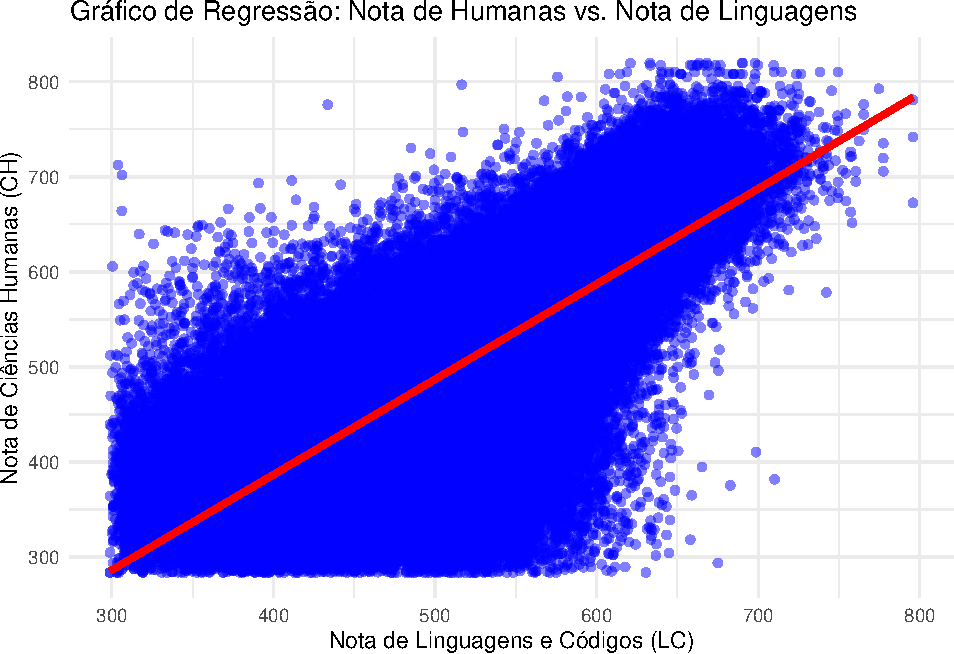
\includegraphics[keepaspectratio]{relatorio_files/figure-latex/unnamed-chunk-5-1.pdf}}

O ``Gráfico de Regressão: Nota de Humanas vs.~Nota de Linguagens''
confirma a correlação positiva. Nesse cenário, os pontos estão
razoavelmente agrupados ao redor da linha vermelha, que sobe da esquerda
para a direita, confirmando a tendência de que notas altas em LC
acompanham notas altas em CH. Para o modelo elaborado, temos a seguinte
equação: Nota\_CH = 93.30 + 0.82 * Nota\_LC. Atraves dessa equação, é
possível dizer que para cada 1 ponto que um aluno ganha em na prova de
linguagens (NU\_NOTA\_LC), espera-se que sua nota em humanas
(NU\_NOTA\_CH) aumente, em média, 0.82 pontos. Logo, é possível afirmar
que a nota de Linguagens em geral consegue prever a nota de Humanas.

\end{document}
